


\section{A few calculations}
\label{sec:examples}

What happens if one desingularizes, say the result of collapsing the second face of a standard $2$-simplex, as in \cref{fig:ch2_Desing_2simpl_collapsed_second_face}? The dashed line segment is meant to indicate that the second face has been collapsed. The dotted lines are meant to illustrate the identifications that arise as a result of the desingularization. The next example is a slight generalization in that it replaces $2$ with $n$ and $\delta _2$ with $\delta _n\cdots \delta _{k+1}$ for some $k$ that replaces $1$. We will use the notion of enforcer from \cref{def:enforcer}.
\begin{example}\label{ex:second_simplest_non-trivial_desingularization}
Let $\mu :[k]\to [n]$ be the face operator defined by
\[\mu =\delta _n\cdots \delta _{k+1}.\]
Consider the cocartesian square
\begin{equation}
\label{eq:first_diagram_ex_second_simplest_non-trivial_desingularization}
\begin{gathered}
\xymatrix{
\Delta [k] \ar[d]_{\mu } \ar[r] & \Delta [0] \ar[d] \\
\Delta [n] \ar[r]_{\bar{x} } & X
}
\end{gathered}
\end{equation}
in $sSet$, in the non-trivial case $0<k<n$. The non-degenerate simplex $x$ is then not embedded. We will argue that
\[DX\cong \Delta [n-k]\]
by use of the decomposition of $X$ as the pushout above.

The enforcer
\[\rho _x=\sigma _0\cdots \sigma _{k-1}\]
of $x$ fits into the commutative solid diagram
\begin{equation}
\label{eq:second_diagram_ex_second_simplest_non-trivial_desingularization}
\begin{gathered}
\xymatrix{
\Delta [k] \ar[d]_{\mu } \ar[r] & \Delta [0] \ar[d] \ar@/^1pc/[ddr]^{\varepsilon _0} \\
\Delta [n] \ar[r]_{\bar{x} } \ar@/_2pc/[drr]_{\rho _x} & X \ar@{-->}[dr] \\
&& \Delta [n-k]
}
\end{gathered}
\end{equation}
in $sSet$, which gives rise to a canonical dashed map $X\to \Delta [n-k]$. Next, consider the diagram
\begin{equation}
\label{eq:third_diagram_ex_second_simplest_non-trivial_desingularization}
\begin{gathered}
\xymatrix{
\Delta [n] \ar[d]_{\bar{x} } \ar[r]^(.40){\rho _x} & \Delta [n-k] \ar[d] \ar@/^1pc/[ddr]^{id} \\
X \ar@/_1pc/[drr] \ar[r] & Y \ar@{-->}[dr] \\
&& \Delta [n-k]
}
\end{gathered}
\end{equation}
in $sSet$ where $X\to \Delta [n-k]$ is the map from (\ref{eq:second_diagram_ex_second_simplest_non-trivial_desingularization}). In (\ref{eq:third_diagram_ex_second_simplest_non-trivial_desingularization}), the simplicial set $Y$ is the pushout
\[Y=X\sqcup _{\Delta [n]}\Delta [n-k].\]
From the triangle on the right it follows that $\Delta [n-k]\to Y$ is degreewise injective and that $Y\to \Delta [n-k]$ is degreewise surjective.

Meanwhile, the map $\Delta [n-k]\to Y$ is a cobase change of the map $\bar{x}$, which is itself a cobase change of the degreewise surjective map $\Delta [k]\to \Delta [0]$, as is seen from (\ref{eq:first_diagram_ex_second_simplest_non-trivial_desingularization}). Hence, the map $\Delta [n-k]\to Y$ is degreewise surjective. It follows that $Y\xrightarrow{\cong } \Delta [n-k]$ is an isomorphism. Thus $Y$ is seen to be non-singular. From \cref{lem:pushout_along_enforcers_intermediate_desingularization}, we get that
\[DX\cong Y\cong \Delta [n-k],\]
which was our claim.
\end{example}
\noindent The computation of $DX$ in \cref{ex:second_simplest_non-trivial_desingularization} was particularly easy because of the unusual decomposition of $X$ which in turn arose partly from the fact that $X$ was generated by a single non-degenerate simplex.

\begin{figure}
\centering
\begin{tikzpicture}[scale=0.4]
% Vertices of a triangle
\coordinate (2) at (90:3cm);
\coordinate (0) at (210:3cm);
\coordinate (1) at (-30:3cm);

% Nodes to mark vertices of a triangle
\node [above] at (2) {2};
\node [below left] at (0) {0};
\node [below right] at (1) {1};

% Draw line between the vertices 0,1 and 2 and name the midpoints
\draw (0.north east)--(2.south) coordinate[midway](02);
\draw [dashed] (0.north east)--(1.north west) coordinate[midway](01);
\draw (1.north west)--(2.south) coordinate[midway](12);

% Illustrate the effect of desingularization
\foreach \s in {1,...,9}
	\draw [dotted] (barycentric cs:0=\s/10,2=1-\s/10)--(barycentric cs:1=\s/10,2=1-\s/10);

\end{tikzpicture}
\caption{Desingularizing the standard $2$-simplex whose second face has been collapsed.}
\label{fig:ch2_Desing_2simpl_collapsed_second_face}
\end{figure}

Let us consider a few models of spheres. The first ones have desingularizations that can be calculated simply by an inspection and ad hoc arguments.
\begin{example}\label{ex:desingularization_model_n-sphere}
Consider the cocartesian square
\begin{displaymath}
\xymatrix{
\partial \Delta [n] \ar[d] \ar[r] & \Delta [0] \ar[d] \\
\Delta [n] \ar[r]_(.35){\bar{x} } & \Delta [n]/\partial \Delta [n]
}
\end{displaymath}
in $sSet$. The non-degenerate simplex $x$ is not embedded if $n>0$. In the case when $n=0$, we get
\[\Delta [0]/\partial \Delta [0]\cong \Delta [0]\sqcup \Delta [0],\]
which is non-singular. In other words, desingularization has no effect on $\Delta [0]/\partial \Delta [0]$. Else if $n>0$, then we can apply \cref{ex:simplest_non-trivial_desingularization} to obtain
\[D(\Delta [n]/\partial \Delta [n])\cong \Delta [0].\]
The latter calculation shows that desingularization has homotopically destructive tendencies.
\end{example}
\noindent We record the results from \cref{ex:desingularization_model_n-sphere} in \cref{tab:Desing_spherical_mod} below, which is explained shortly.

What if we subdivide the model $\Delta [n]/\partial \Delta [n]$ of the $n$-sphere before applying desingularization? Let $Sd$ denote the Kan subdivision. See \cite[Def.~2.2.7]{WJR13} or \cite[p.~148]{FP90} for a definition. The Kan subdivision is the left Kan extension of barycentric subdivision along the Yoneda embedding \cite[p.~37]{WJR13}, so to get a mental picture of its effect one can think of barycentric subdivision. There are illustrations of desingularizations of Kan subdivisions in \cref{fig:ch2_Desing_singlysubd_2simpl} and \cref{fig:ch2_Desing_doublysubd_2simpl}. Note that $Sd$ preserves degreewise injective maps \cite[Cor.~4.2.9]{FP90} and that it has a right adjoint \cite[Prop.~4.2.10]{FP90}. In particular, the Kan subdivision preserves attachings.

At this point, we introduce the \textbf{Barratt nerve} \cite[Def.~2.2.3]{WJR13}
\[BX=N(X^\sharp )\]
of a simplicial set $X$ for comparison with $Sd\, X$. Here, we let the set $X^\sharp$ of non-degenerate simplices have the partial order $\leq$ defined by letting $y\leq x$ if $y$ is a face of $x$. We think of a partially ordered set, poset for short, $(P,\leq )$ as a small category by letting the elements of $P$ be the objects and we let there be a morphism $p\to p'$ if $p\leq p'$. One can interpret $B$ as an endofunctor of simplicial sets, although its image is in the full subcategory $nsSet$. Indeed, the Barratt nerve $BX$, of every simplicial set $X$, is the simplicial set associated with an ordered simplicial complex. There is \cite[p.~37]{WJR13} a natural degreewise surjective \cite[Lem.~2.2.10]{WJR13} map
\[b_X:Sd\, X\to BX,\]
which is an isomorphism if and only if $X$ is non-singular \cite[Lem.~2.2.11]{WJR13}.

\begin{table}
\centering
\begin{tikzpicture}
    \matrix(dict)[matrix of nodes,
    nodes={align=center,text width=8em},
    row 1/.style={anchor=south},
    column 1/.style={nodes={text width=4.5em,align=right}}
    ]{
        $DSd^k(X)$ & $k=0$ & $k=1$ & $k=2$ \\
        $n=0$ & $\Delta [0]\sqcup \Delta [0]$ & $\Delta [0]\sqcup \Delta [0]$ & $\Delta [0]\sqcup \Delta [0]$ \\
        $n=1$ & $\Delta [0]$ & $\Delta [1]\sqcup _{\partial \Delta [1]}\Delta [1]$ & $A\sqcup _{\partial A}A$ \\
        $n=2$ & $\Delta [0]$ & $\Delta [1]$ & $S(12-gon)$ \\
    };
    \draw(dict-1-1.south west)--(dict-1-4.south east);
    \draw(dict-1-1.north east)--(dict-4-1.south east);
\end{tikzpicture}
\caption{Desingularizations of models of certain spheres. Here, we denote $X=\Delta [n]/\partial \Delta [n]$, $A=Sd(\Delta [1])$ and $\partial A=Sd(\partial \Delta [1])$.}
\label{tab:Desing_spherical_mod}
\end{table}

Let $Sd^k$ denote the Kan subdivision applied $k$ times, for each integer $k\geq 0$. We consider $X=Sd^k(\Delta [n]/\partial \Delta [n])$ for $0\leq n\leq 2$ and $0\leq k\leq 2$. As we obtain desingularizations of these simplicial sets, we record the results in \cref{tab:Desing_spherical_mod}. \cref{ex:desingularization_model_n-sphere} took care of the case when $k=0$. Furthermore, we have the following calculations.
\begin{example}\label{ex:all_subdivisions_sphere_dim_zero_coincidence_dim_one}
For every $k\geq 0$, we have
\[Sd^k(\Delta [0]/\partial \Delta [0])\cong \Delta [0]\sqcup \Delta [0].\]
So too, for $k=1$ and $k=2$. Applying desingularization has no effect as $Sd^k(\Delta [0]/\partial \Delta [0])$ is already non-singular. By a coincidence, the simplicial set $Sd(\Delta [1]/\partial \Delta [1])$ is also non-singular, as we explain next.

The commutative square
\begin{displaymath}
\xymatrix{
[0] \ar[d]_{\varepsilon _1} \ar[rr]^{\varepsilon _1} && [1] \ar[d]^{0\mapsto \varepsilon _0,\; 1\mapsto \iota } \\
[1] \ar[rr]_{0\mapsto \varepsilon _1,\; 1\mapsto \iota } && \Delta [1]^\sharp
}
\end{displaymath}
where $\iota$ denotes the identity, gives rise to a canonical map
\[\Delta [1]\sqcup _{\Delta [0]}\Delta [1]\xrightarrow{\cong } B(\Delta [1])\]
that is an isomorphism. Inverting it and forming the composite
\[Sd(\Delta [1])\xrightarrow{b_{\Delta [1]}} B(\Delta [1])\xrightarrow{\cong } \Delta [1]\sqcup _{\Delta [0]}\Delta [1]\]
which is in turn precomposed with the canonical map
\[\Delta [1]\sqcup \Delta [1]\to \Delta [1]\sqcup _{\partial \Delta [1]}\Delta [1]\]
yields the solid diagram
\begin{displaymath}
\xymatrix@=0.9em{
Sd(\partial \Delta [1]) \ar[d] \ar[r] & Sd(\Delta [0]) \ar[d] \ar@/^2pc/[ddr] \\
Sd(\Delta [1]) \ar@/_2pc/[drr] \ar[r] & Sd(\Delta [1]/\partial \Delta [1]) \ar@{-->}[dr]^\cong \\
&& \Delta [1]\sqcup _{\partial \Delta [1]}\Delta [1]
}
\end{displaymath}
that commutes, thus giving rise to a canonical dashed map that is in fact an isomorpism. Then the desingularization is trivially
\[DSd(\Delta [1]/\partial \Delta [1])\cong \Delta [1]\sqcup _{\partial \Delta [1]}\Delta [1],\]
which is also recorded in \cref{tab:Desing_spherical_mod}.
\end{example}
\noindent We resume with slightly more complicated examples.

By \cref{lem:desing_unique_factorization_through_unit}, we obtain a map $t_X:DSd\, X\to BX$. Because $\eta _{Sd\, X}$ and $b_X$ are natural, because $\eta _{Sd\, X}$ is degreewise surjective and because the target of $b_X$ is non-singular, the map $t_X$ can be interpreted as a natural map between functors $sSet\to nsSet$ when we corestrict $B$ to $nsSet$.

We will prove the following result.
\begin{proposition}\label{prop:double_subdivision_sphere_low_dimension}
The map
\[DSd^2(\Delta [n]/\partial \Delta [n])\xrightarrow{t_{Sd(\Delta [n]/\partial \Delta [n])}} BSd(\Delta [n]/\partial \Delta [n])\]
is an isomorphism for $0\leq n\leq 2$.
\end{proposition}
\noindent For the proof of \cref{prop:double_subdivision_sphere_low_dimension}, note we have already taken care of the case when $n=0$ in \cref{ex:all_subdivisions_sphere_dim_zero_coincidence_dim_one}. The case when $n=1$ follows from \cref{ex:double_subdivision_sphere_dim_one} below.
\begin{example}\label{ex:double_subdivision_sphere_dim_one}
By \cref{ex:all_subdivisions_sphere_dim_zero_coincidence_dim_one}, the simplicial set $Sd(\Delta [1]/\partial \Delta [1])$ is non-singular. Therefore the map $b_{Sd(\Delta [1]/\partial \Delta [1])}$ is an isomorphism, which implies that the map
\[t_{Sd(\Delta [1]/\partial \Delta [1])}:DSd^2(\Delta [1]/\partial \Delta [1])\xrightarrow{\cong } BSd(\Delta [1]/\partial \Delta [1])\]
is an isomorphism.
\end{example}
\noindent To prove \cref{prop:double_subdivision_sphere_low_dimension}, it remains to consider the case when $n=2$.

\begin{figure}
\centering
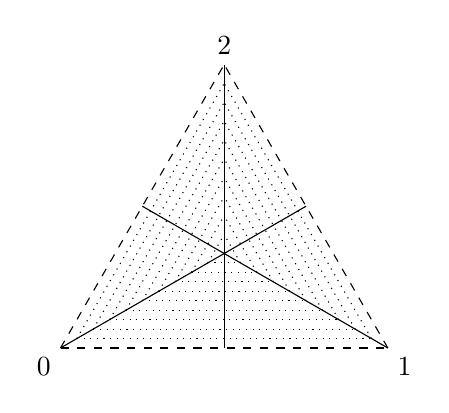
\begin{tikzpicture}[scale=0.8]
% Vertices of a triangle
\coordinate (2) at (90:3cm);
\coordinate (0) at (210:3cm);
\coordinate (1) at (-30:3cm);

% Nodes to mark vertices of a triangle
\node [above] at (2) {2};
\node [below left] at (0) {0};
\node [below right] at (1) {1};

% Draw line between the vertices 0,1 and 2 and name the midpoints
\draw [dashed] (0.north east)--(2.south) coordinate[midway](02);
\draw [dashed] (0.north east)--(1.north west) coordinate[midway](01);
\draw [dashed] (1.north west)--(2.south) coordinate[midway](12);

% Barycenter, could also be found by means of the intersection library of tikz
\coordinate (012) at (barycentric cs:0=1,1=1,2=1);

% Subdivide the 2-simplex
\foreach \x in {(0),(01),(1),(12),(2),(02)}
	\draw (012)--\x;

% Illustrate the effect of desingularization
\foreach \x in {0,1}
	\foreach \y in {1,2}
		\foreach \s in {1,...,9}
			\draw [dotted] (barycentric cs:\x=\s/10,012=1-\s/10)--(barycentric cs:\y=\s/10,012=1-\s/10);

\end{tikzpicture}
\caption{Desingularizing the Kan subdivision of the $2$-simplex with collapsed boundary.}
\label{fig:ch2_Desing_singlysubd_2simpl}
\end{figure}

Before we prove \cref{prop:double_subdivision_sphere_low_dimension} in the case when $n=2$, we contemplate how to desingularize $Sd(\Delta [2]/\partial \Delta [2])$, which is a similar task, although slightly easier. We make use of the notion of enforcer from \cref{def:enforcer}.
\begin{example}\label{ex:desingularization_model_n-sphere_subdivided}
Consider the cocartesian square
\begin{equation}
\label{eq:first_diagram_ex_desingularization_model_n-sphere_subdivided}
\begin{gathered}
\xymatrix{
Sd(\partial \Delta [2]) \ar[d] \ar[r] & Sd(\Delta [0]) \ar[d] \\
Sd(\Delta [2]) \ar[r] & Sd\, X
}
\end{gathered}
\end{equation}
in $sSet$, where we have written $X=\Delta [2]/\partial \Delta [2]$ for brevity. We will prove that
\begin{equation}\label{eq:first_equation_desingularization_model_n-sphere_subdivided}
DSd\, X\cong \Delta [1].
\end{equation}
In \cref{fig:ch2_Desing_singlysubd_2simpl}, we illustrate the effect of desingularizing $Sd\, X$. This illustration indicates the idea of the proof and is helpful in bookkeeping. The dashed line segments that are part of the boundary are meant to indicate that the boundary has been collapsed in order to form $\Delta [2]/\partial \Delta [2]$. The dotted line segments are meant to illustrate how identifications arise when desingularizing.

The simplicial set $Sd\, X$ is generated by six (non-degenerate) $2$-simplices as $Sd(\Delta [2])$ is generated by six non-degenerate $2$-simplices and as
\[Sd(\Delta [2])\to Sd\, X\]
is degreewise surjective. We will name these six generators. Let the simplex $y_1$ be the image under
\[B(\Delta [2])\cong Sd(\Delta [2])\to Sd\, X\]
of the simplex $\{0<01<012\}$. Furthermore, let $y_2$ be the image of the next non-degenerate $2$-simplex $\{1<01<012\}$ as we move counterclockwise in \cref{fig:ch2_Desing_singlysubd_2simpl} and so on up to and including $j=6$. Thus the set
\[\{y_j\} _{j\in J},\, J=\{ 1,\dots ,6\}\]
generates $Sd\, X$.

The simplicial set $Sd(\Delta [2])$ has seven $0$-simplices that correspond to the seven elements of $\Delta [2]^\sharp$. The six $0$-simplices on the boundary $Sd(\partial \Delta [2])$ are identified with each other when $Sd\, X$ is formed from $Sd(\Delta [2])$. However, the $0$-simplex $012$ is not identified with these. Write $z_j=\eta _{Sd\, X}(y_j)$ for each $j\in J$. Each of the $2$-simplices $y_j$, $j\in J$, is such that the vertices $y_j\varepsilon _0$ and $y_j\varepsilon _1$ are on the boundary and that $y_j\varepsilon _2$ is equal to $012$. Thus we see that each of the simplices $y_j$, $j\in J$, has the elementary degeneracy operator
\[\rho _{y_j}=\sigma _0\]
as its enforcer. Let $\rho$ denote this common enforcer.

For each $j\in J$, write $z_j=\eta _{Sd\, X}(y_j)$. From \cref{prop:role_of_enforcers}, we have the commutative square
\begin{equation}
\label{eq:second_diagram_ex_desingularization_model_n-sphere_subdivided}
\begin{gathered}
\xymatrix{
\bigsqcup _{j\in J}\Delta [2] \ar[d]_{\vee _{j\in J}(\bar{y} _j)} \ar[rr]^{\sqcup _{j\in J}(\rho )} && \bigsqcup _{j\in J}\Delta [1] \ar[d]^{\vee _{j\in J}(\bar{w} _j)} \\
Sd\, X \ar[rr]_{\eta _{Sd\, X}} && UDSd\, X
}
\end{gathered}
\end{equation}
in $sSet$, where $w_j$ is the canonical degeneracy of the non-degenerate part of $z_j$, $j\in J$.  In this case, the simplices $w_j$, $j\in J$, are embedded and therefore non-degenerate. This way we see how the simplices $z_j$, $j\in J$, are degenerate.

Because the simplices $z_j$, $j\in J$, are all degenerate it follows that $DSd\, X$ is generated by the images under $\eta _{Sd\, X}$ of the six embedded $1$-simplices of $Sd\, X$. We will argue that all of these images are equal.

Pick a $j\in J$. Two of the six embedded $1$-simplices of $Sd\, X$ are the faces $y_j\delta _1$ and $y_j\delta _0$ of $y_j$. Because $\delta _1$ and $\delta _0$ are both sections of $\rho$, we get that
\begin{displaymath}
\begin{array}{rclclcl}
z_j\delta _1 & = & (w_j\rho )\delta _1 & = & w_j(\rho \delta _1) & = & w_j \\
z_j\delta _0 & = & (w_j\rho )\delta _0 & = & w_j(\rho \delta _0) & = & w_j.
\end{array}
\end{displaymath}
Thus it follows that the image under $\eta _{Sd\, X}$ of each of the faces $y_j\delta _1$ and $y_j\delta _0$ is equal to $w_j$. Let us express this with $y_j\delta _1\sim y_j\delta _0$ for each $j\in J$.

By moving counterclockwise in \cref{fig:ch2_Desing_singlysubd_2simpl}, we get that
\begin{displaymath}
\begin{array}{rclcl}
y_1\delta _0 & = & y_2\delta _0 & \sim & y_2\delta _1 \\
y_2\delta _1 & = & y_3\delta _1 & \sim & y_3\delta _0 \\
y_3\delta _0 & = & y_4\delta _0 & \sim & y_4\delta _1 \\
y_4\delta _1 & = & y_5\delta _1 & \sim & y_5\delta _0 \\
y_5\delta _0 & = & y_6\delta _0 & \sim & y_6\delta _1.
\end{array}
\end{displaymath}
This shows that
\[w_1=w_2=\cdots =w_6,\]
implying that (\ref{eq:first_equation_desingularization_model_n-sphere_subdivided}) holds.
\end{example}
\noindent To complete \cref{tab:Desing_spherical_mod}, the only remaining case is when $k=2$ and $n=2$.

Note that the functor $BSd$ replaces a simplicial set with an ordered simplicial complex of the same homotopy type \cite[Ex.~3--8, pp.~219--220]{FP90}. To conjecture the homotopical content of the claim of \cref{prop:double_subdivision_sphere_low_dimension} one uses the sort of intuition that comes from knowledge of regular neighborhood theory, as explained in \cite[§3]{RS72} or \cite[§II]{Hu69}. For example, the reason that collapsing the boundary of $Sd^k(\Delta [2])$ in the category $nsSet$ is an operation that preserves the homotopy type in the case when $k=2$, but not in the case when $k=1$ is indicated and illustrated in a remark in \cite[p.~51]{Hu69}. It turns out that the double subdivision creates a sufficiently nice neighborhood around the boundary. \cref{fig:ch2_Desing_doublysubd_2simpl}, which is used for bookkeeping in the proof of \cref{prop:double_subdivision_sphere_low_dimension}, illustrates the phenomenon.  

% Takes advantage of barycentric coordinates and for loops. Can surely be more elegant.
\begin{figure}
\centering
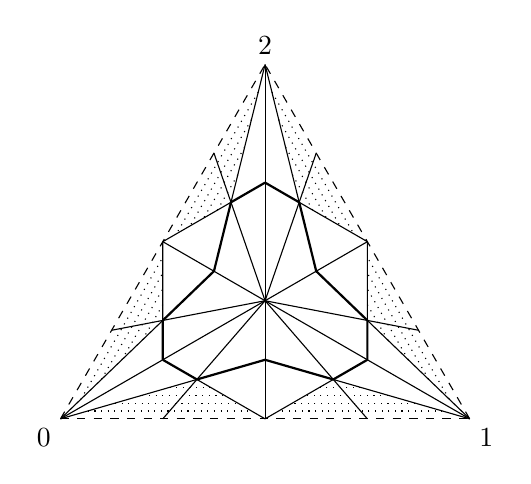
\begin{tikzpicture}

% Vertices of a triangle
\coordinate (2) at (90:3cm);
\coordinate (0) at (210:3cm);
\coordinate (1) at (-30:3cm);

% Nodes to mark vertices of a triangle
\node [above] at (2) {2};
\node [below left] at (0) {0};
\node [below right] at (1) {1};

% Draw line between the vertices 0,1 and 2 and name the midpoints
\draw [dashed] (0.north east)--(2.south) coordinate[midway](02);
\draw [dashed] (0.north east)--(1.north west) coordinate[midway](01);
\draw [dashed] (1.north west)--(2.south) coordinate[midway](12);

% Barycenter, could also be found by means of the intersection library of tikz
\coordinate (012) at (barycentric cs:0=1,1=1,2=1);

% Draws lines from vertices of original triangle to barycentre of original triangle and...
\draw (0.north east)--(012) coordinate[midway](0<012);
\draw (1.north west)--(012) coordinate[midway](1<012);
\draw (2.south)--(012) coordinate[midway](2<012);
\draw (01)--(012) coordinate[midway](01<012);
\draw (12)--(012) coordinate[midway](12<012);
\draw (02)--(012) coordinate[midway](02<012);

% Subdivide each of the six new 2-simplices. To highlight the structure of the desingularized simplicial set we make certain lines thicker
\coordinate (0<01<012) at (barycentric cs:0=1,01=1,012=1);
\coordinate (0<01) at (barycentric cs:0=0.5,01=0.5);
\foreach \x in {(0),(0<01),(01),(012)}
	\draw (0<01<012)--\x;
\foreach \x in {(0<012),(01<012)}
	\draw [thick] (0<01<012)--\x;

\coordinate (1<01<012) at (barycentric cs:1=1,01=1,012=1);
\coordinate (1<01) at (barycentric cs:1=0.5,01=0.5);
\foreach \x in {(1),(1<01),(01),(012)}
	\draw (1<01<012)--\x;
\foreach \x in {(01<012),(1<012)}
	\draw [thick] (1<01<012)--\x;

\coordinate (1<12<012) at (barycentric cs:1=1,12=1,012=1);
\coordinate (1<12) at (barycentric cs:1=0.5,12=0.5);
\foreach \x in {(1),(1<12),(12),(012)}
	\draw (1<12<012)--\x;
\foreach \x in {(12<012),(1<012)}
	\draw [thick] (1<12<012)--\x;

\coordinate (2<12<012) at (barycentric cs:2=1,12=1,012=1);
\coordinate (2<12) at (barycentric cs:2=0.5,12=0.5);
\foreach \x in {(2),(2<12),(12),(012)}
	\draw (2<12<012)--\x;
\foreach \x in {(12<012),(2<012)}
	\draw [thick] (2<12<012)--\x;
	
\coordinate (2<02<012) at (barycentric cs:2=1,02=1,012=1);
\coordinate (2<02) at (barycentric cs:2=0.5,02=0.5);
\foreach \x in {(2),(2<02),(02),(012)}
	\draw (2<02<012)--\x;
\foreach \x in {(02<012),(2<012)}
	\draw [thick] (2<02<012)--\x;
	
\coordinate (0<02<012) at (barycentric cs:0=1,02=1,012=1);
\coordinate (0<02) at (barycentric cs:0=0.5,02=0.5);
\foreach \x in {(0),(0<02),(02),(012)}
	\draw (0<02<012)--\x;
\foreach \x in {(02<012),(0<012)}
	\draw [thick] (0<02<012)--\x;

% Effect of desingularizing doubly subdivided 2-simplex with collapsed boundary. We make these lines dotted.
\foreach \x in {0.2,0.4,0.6,0.8}
	\draw [dotted] (barycentric cs:0=\x,0<01<012=1-\x)--(barycentric cs:01=\x,0<01<012=1-\x);

\foreach \x in {0.2,0.4,0.6,0.8}
	\draw [dotted] (barycentric cs:1=\x,1<01<012=1-\x)--(barycentric cs:01=\x,1<01<012=1-\x);

\foreach \x in {0.2,0.4,0.6,0.8}
	\draw [dotted] (barycentric cs:1=\x,1<12<012=1-\x)--(barycentric cs:12=\x,1<12<012=1-\x);

\foreach \x in {0.2,0.4,0.6,0.8}
	\draw [dotted] (barycentric cs:2=\x,2<12<012=1-\x)--(barycentric cs:12=\x,2<12<012=1-\x);

\foreach \x in {0.2,0.4,0.6,0.8}
	\draw [dotted] (barycentric cs:2=\x,2<02<012=1-\x)--(barycentric cs:02=\x,2<02<012=1-\x);

\foreach \x in {0.2,0.4,0.6,0.8}
	\draw [dotted] (barycentric cs:0=\x,0<02<012=1-\x)--(barycentric cs:02=\x,0<02<012=1-\x);
\end{tikzpicture}
\caption{Desingularizing the double Kan subdivision of the standard $2$-simplex with collapsed boundary.}
\label{fig:ch2_Desing_doublysubd_2simpl}
\end{figure}

We are ready to prove the proposition. The method is similar to that of \cref{ex:desingularization_model_n-sphere_subdivided}.
\begin{proof}[Proof of \cref{prop:double_subdivision_sphere_low_dimension}.]
We will argue that
\begin{equation}
\label{eq:first_expression_proof_of_prop_double_subdivision_sphere_low_dimension}
DSd^2\, X\cong S(12-gon)
\end{equation}
where $X=\Delta [2]/\partial \Delta [2]$. By this, we mean that $DSd^2\, X$ is the suspension of a $12$-gon, which is what $BSd\, X$ is. As the cases when $n=0$ and $n=1$ were taken care of by \cref{ex:all_subdivisions_sphere_dim_zero_coincidence_dim_one} and \cref{ex:double_subdivision_sphere_dim_one}, respectively, the argument below finishes the proof.

To study $DSd^2\, X$ is to study the diagram that we get by applying $Sd$ to (\ref{eq:first_diagram_ex_desingularization_model_n-sphere_subdivided}). For an illustration of the formation of $DSd^2\, X$ from $Sd^2\, X$, see \cref{fig:ch2_Desing_doublysubd_2simpl}. We use the same conventions as in \cref{fig:ch2_Desing_singlysubd_2simpl} and one additional convention. Namely, there are exactly twelve line segments that are thicker than the others. These form the $12$-gon we mentioned. The simplicial set $BSd\, X$ is the nerve of the poset
\begin{equation}
\label{eq:first_diagram_proof_prop_double_subdivision_sphere_low_dimension}
\begin{gathered}
\xymatrix@=0.6em{
&&&&&& [012] \\
\\
\\
&&&&&& \bullet \ar@{..>}[lllld] \ar@{<-}[uuu] \ar@/^0.3pc/@{<..}[ddddddddd] \ar@{..>}[drrrr] \\
&& \bullet \ar@{<..}[ddddddddrrrr] \ar@{<-}[uuuurrrr] &&&&&&&& \bullet \ar@{<..}[lllldddddddd] \ar@{<-}[lllluuuu] \\
&& \bullet \ar@{..>}[lld] \ar@{<..}[dddddddrrrr] \ar@{..>}[u] \ar@{<-}[uuuuurrrr] &&&&&&&& \bullet \ar@{<-}[lllluuuuu] \ar@{..>}[u] \ar@{<..}[llllddddddd] \ar@{..>}[drr] \\
\bullet \ar@{<..}[ddddddrrrrrr] \ar@{<-}[uuuuuurrrrrr] &&&&&&&&&&&& \bullet \ar@{<-}[lllllluuuuuu] \ar@{<..}[lllllldddddd] \\
\bullet \ar[u] \ar@{<-}[dddddrrrrrr] \ar@{<-}[uuuuuuurrrrrr] \ar[drr] &&&&&& \bullet \ar[lllld] \ar@/^0.3pc/@{<-}[uuuuuuu] \ar[drrrr] &&&&&& \bullet \ar[lld] \ar@{<-}[llllllddddd] \ar@{<-}[lllllluuuuuuu] \ar[u] \\
&& \bullet \ar@{<-}[ddddrrrr] \ar@{<-}[uuuuuuuurrrr] &&&&&&&& \bullet \ar@{<-}[lllluuuuuuuu] \ar@{<-}[lllldddd] \\
\\
\\
\\
&&&&&& [0] \ar[uuuuu]
}
\end{gathered}
\end{equation}
namely $Sd(X)^\sharp$. In (\ref{eq:first_diagram_proof_prop_double_subdivision_sphere_low_dimension}) we have drawn the $0$-simplex $012$ as the cone point at the top.

The cone point at the bottom, which we denote $[0]$, is the $0$-simplex that is the result of the identifications
\[0\sim 01\sim 1\sim 12\sim 2\sim 02.\]
These names arise in an intuitive manner from considering the poset $\Delta [2]^\sharp$ whose objects correspond to the $0$-simplices of
\[B(\Delta [2])\cong Sd(\Delta [2])\]
whose non-degenerate simplices in turn correspond to the $0$-simplices of
\[B^2(\Delta [2])\cong BSd(\Delta [2])\cong Sd^2(\Delta [2]).\]
For example, the object $0$ arises from $\varepsilon _0$ and $1$ from $\varepsilon _1$. Furthermore, the object $02$ arises from $\delta _1$. The objects of the poset $Sd(X)^\sharp$ that are not cone points are the non-degenerate $1$-simplices of $Sd\, X$, of which there are six, and the non-degenerate $2$-simplices, of which there are also six.

We proceed by naming the twelve non-embedded non-degenerate $2$-simplices of $Sd^2\, X$. First, we let $y_1$ be the image of
\[\{ \{0\} <\{0<01\} <\{0<01<012\} \}\]
under $Sd^2(\Delta [2])\to Sd^2\, X$. Next, we let $y_2$ be the image of the next $2$-simplex as we move counterclockwise in \cref{fig:ch2_Desing_doublysubd_2simpl} up to and including $j=12$. Write $J=\{ 1,\dots ,12\}$. Each of the simplices $y_j$, $j\in J$, has the elementary degeneracy operator
\[\rho _{y_j}=\sigma _0\]
as its enforcer. Let $\rho$ denote this common enforcer.

From \cref{prop:role_of_enforcers}, we have the cocartesian square
\begin{equation}
\label{eq:second_diagram_proof_prop_double_subdivision_sphere_low_dimension}
\begin{gathered}
\xymatrix{
\bigsqcup _{j\in J}\Delta [2] \ar[d]_{\vee _{j\in J}(\bar{y} _j)} \ar[rr]^{\sqcup _{j\in J}(\rho )} && \bigsqcup _{j\in J}\Delta [1] \ar[d] \\
Sd^2\, X \ar[rr] && Z
}
\end{gathered}
\end{equation}
in $sSet$. Let $z_j$, $j\in J$, be the image of $y_j$ under $Sd^2\, X\to Z$. Suppose $z_j=w_j\rho$ for some simplex $w_j$, $j\in J$. Then $w_j$ is embedded as $Sd^2\, X\to Z$ is injective in degree $0$.

The elementary face operators $\delta _1$ and $\delta _0$ are both sections of $\rho$, so we have
\begin{displaymath}
\begin{array}{rclclcl}
z_j\delta _1 & = & (w_j\rho )\delta _1 & = & w_j(\rho \delta _1) & = & w_j \\
z_j\delta _0 & = & (w_j\rho )\delta _0 & = & w_j(\rho \delta _0) & = & w_j.
\end{array}
\end{displaymath}
for each $j\in J$. It follows that the image under $Sd^2\, X\to Z$ of each of the faces $y_j\delta _1$ and $y_j\delta _0$ is equal to $w_j$. Let us express this with $y_j\delta _1\sim y_j\delta _0$.

Suppose $j\in J$ odd. Then
\[y_j\delta _1\sim y_j\delta _0=y_{j+1}\delta _0\sim y_{j+1}\delta _1.\]
Thus we observe that $w_j=w_{j+1}$. We get that $Z$ is non-singular by the bookkeeping performed with the aid of \cref{fig:ch2_Desing_doublysubd_2simpl}. From \cref{lem:pushout_along_enforcers_intermediate_desingularization}, it follows that the simplicial set $Z$ is the desingularization of $Sd^2\, X$. Moreover, the simplicial set $Z$ is the nerve of (\ref{eq:first_diagram_proof_prop_double_subdivision_sphere_low_dimension}). The naturality of $t_{Sd\, X}$ shows that it is an isomorphism.
\end{proof}
























